\documentclass[a4paper,12pt]{report}
% Packages et configuration du header
\NeedsTeXFormat{LaTeX2e}
 
%%%%%%%%%%%%%%%%%%%%%%%%%%%%%%%%%%%%%%%%%%%%%%%%%%%%%%%%%%%%%%%%%%%%
%                          P A C K A G E S                         %
%%%%%%%%%%%%%%%%%%%%%%%%%%%%%%%%%%%%%%%%%%%%%%%%%%%%%%%%%%%%%%%%%%%%

\usepackage[french]{babel}
\usepackage{lmodern}
\usepackage[utf8]{inputenc}
\usepackage[T1]{fontenc}
\usepackage{lipsum}
\usepackage{amsmath}
\usepackage{amssymb}
\usepackage{mathtools}
\usepackage{graphicx}
\usepackage{xspace}
\usepackage{hyperref}
\usepackage{changepage}
\usepackage[kerning=true]{microtype}
\usepackage{csquotes}
\usepackage{tikzpagenodes}
\usepackage{geometry}
\usepackage{enumitem}
\usepackage{fancyhdr}
\usepackage{calc}
\usepackage{tikz}
\usepackage{adjustbox}
\usepackage{pifont}

\usepackage{paper/imtneStyles/imtneChapitre}
\usepackage{paper/imtneStyles/imtnePageDeGarde}

%%%%%%%%%%%%%%%%%%%%%%%%%%%%%%%%%%%%%%%%%%%%%%%%%%%%%%%%%%%%%%%%%%%%%
%                            C O L O R S                            %
%%%%%%%%%%%%%%%%%%%%%%%%%%%%%%%%%%%%%%%%%%%%%%%%%%%%%%%%%%%%%%%%%%%%%

\definecolor{imtneAmbre}{HTML}{fbba00}
\definecolor{imtneAmbreText}{HTML}{f0ab00}
\definecolor{imtneCeleste}{HTML}{00b8de}
\definecolor{imtneMarine}{HTML}{001f41}
\definecolor{imtneMarineText}{HTML}{09192b}
\definecolor{imtneGris}{HTML}{eaeaea}
\color{imtneMarineText}

%%%%%%%%%%%%%%%%%%%%%%%%%%%%%%%%%%%%%%%%%%%%%%%%%%%%%%%%%%%%%%%%%%%%%
%              G E O M E T R Y   A N D   W I D G E T S              %
%%%%%%%%%%%%%%%%%%%%%%%%%%%%%%%%%%%%%%%%%%%%%%%%%%%%%%%%%%%%%%%%%%%%%

\geometry{
  twoside=true,
  head=42.09433pt,
  paperwidth=8.5in,
  paperheight=11in,
  columnsep=2pc,
  top=90pt,
  bottom=65pt,
  inner=50pt,
  outer=50pt,
  marginparwidth=2pc,
  heightrounded
}

\setitemize[1]{label=\textcolor{imtneCeleste}{\ding{228}}}
\setitemize[2]{label=\textbullet}
\setenumerate[1]{font=\bf\color{imtneCeleste}}
\setenumerate[2]{font=\color{imtneMarine}}

\fancyhead[L]{
\includegraphics[width=2cm]{paper/figures/imtne.png}}
\fancyhead[R]{\rightmark}

\newcommand{\authornamefooter}{Shaw E.}
\fancyfoot[LO]{\authornamefooter}
\fancyfoot[LE]{\authornamefooter}

%%%%%%%%%%%%%%%%%%%%%%%%%%%%%%%%%%%%%%%%%%%%%%%%%%%%%%%%%%%%%%%%%%%%%
%                           M A C R O S                             %
%%%%%%%%%%%%%%%%%%%%%%%%%%%%%%%%%%%%%%%%%%%%%%%%%%%%%%%%%%%%%%%%%%%%%

% \newcommand{\g}{Google Nearby Connections\xspace}
% \newcommand{\cl}{\textsc{ClickLeague}\xspace}

\def\imtneGetEltSize{%
  \ifdim \paperwidth < \paperheight
    \paperwidth/10
  \else
    \paperheight/10
  \fi%
}

\newcommand{\annote}[3]{{%
  \footnotesize\sffamily%
  \colorbox{#3}{\bfseries\textcolor{white}{#2}}\hspace{-0.3ex}%
  {\color{#3}%
    $\blacktriangleright$%
    \textit{#1}%
    $\blacktriangleleft$%
  }%
}}

\newcommand{\todo}[1]{\annote{#1}{Todo}{imtneAmbreText}}
\newcommand{\td}{\annote{}{}{imtneAmbreText}}
\newcommand{\note}[1]{\annote{#1}{Note}{imtneGris}}

\makenoidxglossaries
\newglossaryentry{rootserver}{
    name={root name server}, 
    description={13 serveurs faisant autorité sur la racine d’internet et contenant donc les informations sur tous les TLD. Ils sont constitués de 1708 instances (serveur physiques) gérés par 12 opérateurs indépendants et répartis partout dans le monde.}, 
    plural={root name servers}*
}

\newglossaryentry{autoritativeserver}{
    name={serveur faisant autorité}, 
    description={Un serveur faisant autorité sur une zone DNS est un serveur dont les réponses concernant la zone sont considérées comme fiables à l’instant où elle est reçue. (Une réponse qui est gardée en mémoire n’est pas forcément à jour contrairement à une réponse venant directement du serveur faisant autorité)}, 
    plural={serveurs faisant autorité}
}

\newglossaryentry{tld}{
    name={tld},
    description={ou Top Level Domain (nom de domaine de premier niveau) est la partie a la fin d'un nom de domaine tel que le .com .net ou .fr}
}

\newglossaryentry{icann}{
    name={icann},
    description={ ou Internet Corporation for Assigned Names and Numbers est une société à but on lucratif et d'utilité publique consacré à la sécurité, la stabilité et l'interopérabilité de l'internet, elle est responsable de la coordination du système de nommage de l'internet et a donc un impact important sur l'évolution de l'internet}
}
\newglossaryentry{centr}{
    name={centr},
    description={ ou Concil of European National Top-Level domain Registries (Conseil des Registres de Premier Niveau Européens), c'est une association constitué de 52 Registres membres et 9 associés qui sont ensembles responsables de plus de 80\% des noms de domaine enregistrés dans le monde. Son objectif est de promouvoir et participer au développement de nouveau standards et meilleures pratiques}
}
\newglossaryentry{wsis}{
    name={wsis},
    description={ (World Summit on the Information Society), Sommet mondial sur la société de l'information (SMSI) en français est un forum mondial organisé par l'Union Internationale des Télécommunications, une agence de l'Organisation des Nations Unies (ONU). Il vise à réduire l'inégalité des habitants de la planète vis-à-vis de l'accès à l'information par le biais des nouvelles technologies de l'information et de la communication, en particulier d'Internet.}
}

\newglossaryentry{ietf}{
    name={ietf},
    description={ ou Internet Engineering Task Force est l'organisation responsable de la création des standards qui constituent les différents protocole de l'internet au travers des différents RFC}
}
\newglossaryentry{ripencc}{
    name={ripe ncc},
    description={ (Réseaux IP Européens - Network Coordination Centre), un registre régional d'adresses IP. Il dessert l'Europe et une partie de l'Asie, notamment au Moyen-Orient. Il est responsable de l'attribution des adresses IPv4, adresses IPv6,et des numéros d'Autonomous System (ASN) utilisés pour le routage entre opérateurs (utilisation du protocole BGP).}
}

\newglossaryentry{scrape}{
    name={scrape},
    description={processus consistant a extraire des données d'une page web}
}

\newglossaryentry{anycast}{
    name={nuage anycast},
    description={infrastructure internet consistant de plusieurs serveurs possédant la même adresse qui fait que le serveur le plus proche de l'utilisateur répond ce qui permet de grandement réduire le temps de réponse, la charge en bande passante et l'impact des attaques par déni de service ou DoS. (l'afnic et de nombreux autres organismes utilisent cette technologie depuis plus de 10 ans) \cite{anycastAFNIC} \cite{anycastRFC}} 
}



\begin{document}

% Page de garde

  \clearpage
  \newgeometry{top=30pt, bottom=30pt, inner=20pt, outer=30pt}
  \thispagestyle{empty} % Pas de header, footer ou numéro de page

  
  \begin{flushright}
  \begin{minipage}[t]{0.30\textwidth}
      \vspace{4.50cm}
AFNIC\\
1 Rue George Stephenson,\\
78180 Montigny-le-Bretonneux
  \end{minipage}
\end{flushright}
\vspace{0.50cm}
  {\centering\color{imtneAmbreText}\fontsize{40}{48}\selectfont\bfseries \hspace{0pt} Impact energétique du DNS \par}
  \vspace{0.5cm}
  {\centering\color{imtneAmbreText}\Large\bfseries  \hspace{0pt}Découverte de domaine (CI1) \par}
\begin{figure}[!htbp]
  \centering
  \begin{minipage}[t]{0.90\textwidth}
  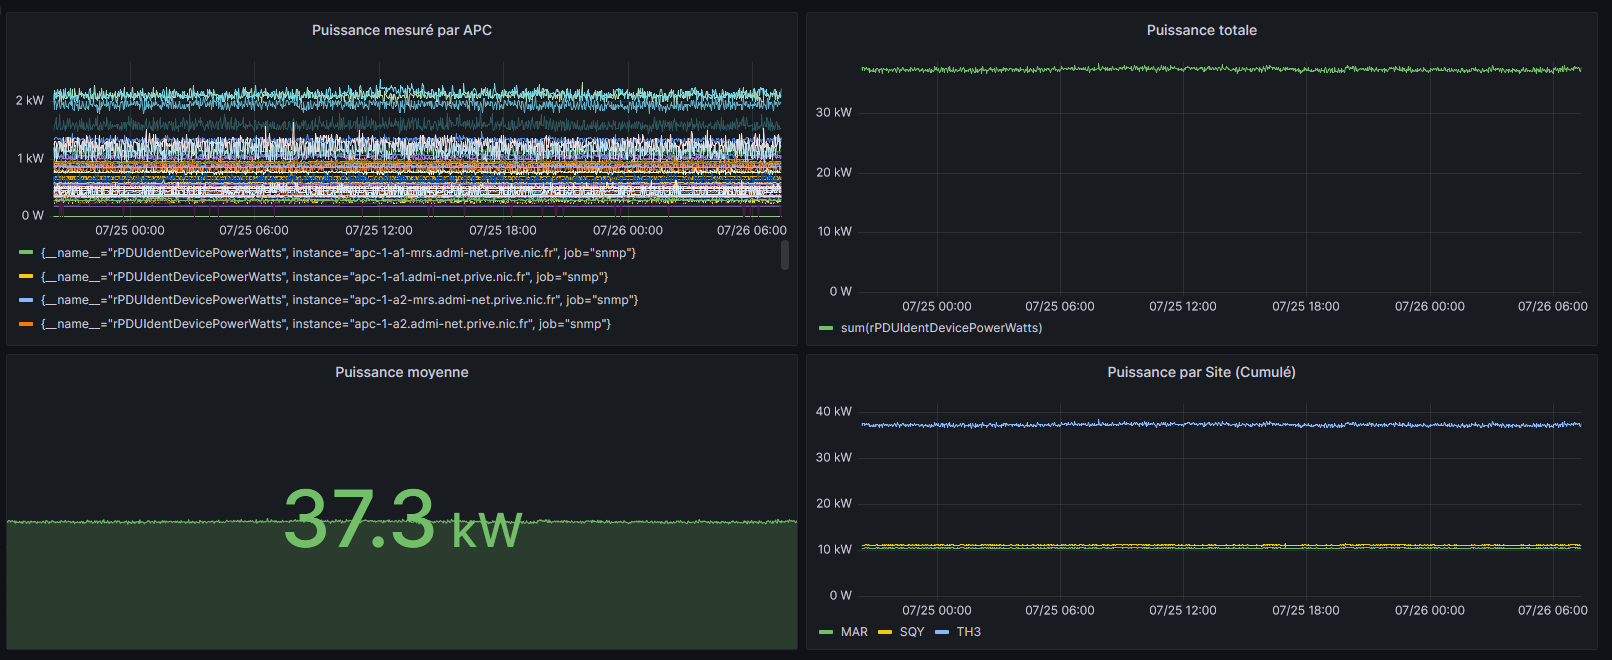
\includegraphics[width=\textwidth]{paper/figures/GrafanaAPC.png}
  \label{fig:pageDeGarde}
  \end{minipage}
\end{figure}

  \vfill

\begin{minipage}[t]{0.65\textwidth}
\vspace{7pt}
Tuteur entreprise : Benoit Ampeau, Directeur Partenariat et Inovation

Référent stage IMT Nord Europe : Aucune Idée
\end{minipage}
\begin{minipage}[t]{0.30\textwidth}
\begin{flushright}
\textbf{Victor Berhault}\\
FISE 2025\\
2022/2023
\end{flushright}
\end{minipage}


  \begin{tikzpicture}[overlay, remember picture]
    \node[anchor=north west] at (current page.north west) {
\includegraphics[height=5cm]{paper/figures/imtne.png}};
    \node[anchor=north east] at (current page.north east) {
\includegraphics[height=5.5cm]{paper/figures/logoOrga.jpg}};
  \end{tikzpicture}
  
  \clearpage
  \restoregeometry % Rétablir la géométrie par défaut
\pagestyle{fancy}



     
\todo{vrai page de garde pour rapport de stage} \\
\todo{consignes : \url{https://partage.imt.fr/index.php/apps/onlyoffice/s/Rqx8xykyxNewzGN}}

\imtnechapitre{Remerciements}
Remerciements Blabla

\todo{Rajouter que les données APC c'est que TH3 + MRS + SQY et pas tout le nuage (donc hébergent aussi d'autres trucs que les serveurs dns)}
\pagebreak
% Table des matières
\tableofcontents

\pagebreak
\setlength{\parskip}{\baselineskip} %espace entre les paragraphes

% Content
\imtnechapitre{Résumés et Mots clés}
\section{Résumé en Français}
J'ai effectué un stage de 16 semaines à l'AFNIC (18 Millions d'euros de CA en 2021 et 91 employés), le registre français responsable de la gestion des noms de domaines finissant notement en .fr, .ovh, .paris et autre.
Dans le contexte de ce stage j'ai intégré l'équipe Labs principalement responsable de la R\verb|&|D.

L'objet principal de ce stage a été la conception et mise en place d'un système de monitoring afin de pouvoir avoir des données sur l'impact énergétique du DNS.
Pour cela j'ai modifié le docker-compose qui constitue le resolveur utilisé en interne afin d'activer les différentes options de monitoring, d'intégrer les outils nécéssaires et d'ouvrir les différents flux, j'ai ensuite récupéré les données avec Prometheus avant de créer des graphiques sur Grafana.

Une autre mission que j'ai eu était de trouver un moyen de relier tous les Wattmetres connectés aux serveurs de production au serveur Grafana interne afin de pouvoir centraliser les données 

\section{Mots Cléfs}
DNS, Monitoring, Docker, Grafana, Prometheus, Scaphandre, RSE
\section{Executive Summary in English}
\todo{Quand Résumé en FR validé}
\section{Key Words}
DNS, Monitoring, Docker, Grafana, Prometheus, Scaphandre, CSR

\imtnechapitre{Introduction}
Après ma 3\textsuperscript{ème} à l'IMT (Institut Mines Telecom) Nord Europe anciennement IMT Lille Douai, j'ai effectué un stage de découverte de dommaine à l'AFNIC.

Ce stage s'est déroulé du 15 Mai au 31 Aout (soit 16 semaines) principalement dans les locaux de l'entreprise a Saint-Quentin-En-Yvelines (en périphérie de Paris) sous la responsabilité de Benoit Ampeau, Directeur Partenariat et Innovation et mon tuteur de stage.

Le sujet de ce stage était de concevoir et développer un système permétant de monitorer les différentes informations liés a un résolveur DNS dont les plus intéréssantes sont la consommation éléctrique en temps réel du serveur et la quantité de requêtes traités par le serveur.
Le but de cette mission est de pouvoir développer la connaissance de l'impact énergétique du DNS ce qui est nécéssaire pour la politique RSE de l'association et servira de base à des papiers ou présentations destinnées aux instances internationnales de la gouvernance et du développement de l'internet.

Pour pouvoir mener a bien cette mission, j'avais a disposition :
\begin{itemize}
    \item L'aide des autres membres de l'équipe Labs dont je faisait partie qui maitrisent l'architecture informatique interne et qui ont donc pus m'aider a choisir et implémenter les différentes solutions.
    \item Un accès sudo (administrateur) à tous les serveurs Labs
    \item Un accès a toute la documentation, au Gitlab et aux autres outils internes a l'AFNIC
\end{itemize}


\imtnechapitre{Contexte}
\setcounter{section}{0}
\section{Présentation Générale de l'organisation}\cite{infoAfnic}
Née en 1997, l’AFNIC est l’Association Française pour le Nommage Internet en Coopération.
Depuis son origine, elle assure la gestion du registre des noms de domaine en France (plus de 4 millions de noms de domaine en .fr à ce jour), en lien avec l’ensemble de l’écosystème de l’internet en France.
Parce que le .fr est un bien public, le rôle de l’AFNIC s’inscrit dans une mission d’intérêt général et d’opérateur de service essentiel qui consiste à contribuer au quotidien :
\begin{itemize}
    \item A un internet sûr et stable ;
    \item Ouvert aux innovations ;
    \item Où la communauté internet française joue un rôle de premier plan.
\end{itemize}

Outre le .fr, l’AFNIC opère également des extensions pour certains territoires ultramarins (comme le .re depuis 2001 pour l’Ile de la Réunion), et depuis 2014 elle est opérateur technique de nouvelles extensions personnalisées (gTLD). Avec des solutions techniques de registre et AFNIC Conseil, l’association a développé une gamme complète pour accompagner les marques et les territoires qui souhaitent se doter de leur propre extension.

Avec une expertise reconnue dans les infrastructures sous-jacentes de l’internet et notamment le DNS (système des noms de domaine), l’AFNIC prend part à la gouvernance mondiale de l’internet, pour définir les règles et les standards de demain.
Association à but non lucratif, l’AFNIC s’est dotée d’une gouvernance multipartite associant toutes les parties prenantes de l’internet en France : pouvoirs publics, utilisateurs et secteur
privé.
Pour défendre l’intérêt général, l’AFNIC protège son indépendance. Elle ne reçoit aucune subvention de fonctionnement, et œuvre comme une PME (effectif de 91 salariés). Le financement de l’activité est entièrement assuré par la mise à disposition de ses prestations.

\section{Ses Membres}
L’AFNIC étant une association, elle est composée de différents membres :
\begin{itemize}
    \item Des représentants des pouvoirs publics
    \item Des bureaux d’enregistrement 
    \item Des personnes morales (associations d’utilisateurs, etc.)
    \item Des personnes physiques (particuliers)
    \item Des associations/organisation nationales ou internationales
\end{itemize}
\vspace{10pt}
Ces membres sont séparés en trois groupes distincts :

\begin{itemize}
    \item Les bureaux d’enregistrement
    \item Les membres utilisateurs (personnes morales ou particuliers)
    \item Les membres correspondants (Collège International) 
\end{itemize}

\section{Ses Missions}
Les missions de l’AFNIC (telles que définies dans ses statuts) ont globalement pour but de favoriser le développement de l’internet en France.
Plus précisément, ses responsabilités sont :
\begin{itemize}
    \item L’Attribution et la Gestion les noms de domaines dont elle est responsable.
    \item Le transfert (au plan National et International) de ses connaissances et de son savoir faire
    \item Le soutiens au développement d’internet, à la formation et à la sensibilisation à ses usages
    \item Toute autre mission qui lui aura été confiée par les pouvoirs publics dans le cadre de la gestion de l’Internet.
\end{itemize}
L’AFNIC doit aussi reverser 90 \verb|%| des bénéfices de la gestion du .fr à sa Fondation AFNIC pour la solidarité numérique.
Du fait de sa position entre Fournisseurs d’Accès Internet (FAI), Utilisateurs et Autorités Publiques, l’AFNIC est impliqué dans l’évolution de la gouvernance et gestion d’internet au niveau international. Plus précisément, elle :
\begin{itemize}
    \item Participe à la gouvernance globale de l'internet (\GLS{icann}, \GLS{centr}, \GLS{wsis}).
    \item Introduire de nouveaux standards et services (\GLS{ietf}, \GLS{ripencc}).
    \item Transmettre des connaissances et savoir-faire (Collège International de l’AFNIC).
\end{itemize}

\todo{Infos RH, CSE, RSE, etc}

\section{Politique RH et RSE}
L'Afnic a un rythme de travail plutôt spécial, au lieu de travailler 35h en 5 jours, tous les employés travaillent en format 32h en 4 jours (ou 3 jours + 2 demi-journées) sans horaires d'arrivée et de départ fixes (certains préfèrent commencer a 7h et finir a 16h pour éviter les embouteillages et profiter de la fin d'après-midi et d'autres préfèrent faire 10h-19h).
En plus de cela, les employés prennent en général 1 jour de télétravail par semaine.
Cela permet une flexibilité du travail bien plus importante que des horaires de travail classique.




\begin{figure}[ht]
  \noindent
  \begin{minipage}{.6\textwidth}
Pour ce qui est de sa politique RSE, l’Afnic s’est engagée dans la convention signée avec l'Etat en juillet 2012 à évaluer son emprunte carbone à publier les résultats de son Bilan Carbone tous les 3 ans.
    
Cette convention a été renouvelle en 2022 avec quelques changements, l'AFNIC "s'engage à réaliser, au minimum tous les deux ans un bilan carbone" et elle "s'engage à ateindre la neutralité carbone de ses activités à travers la mise en place d'un plan de réduction des Gaz à effet de serre (PRGES) et une politique de compensation carbone.
\cite{conventionAfnic2022}
  \end{minipage}
  \hfill
  \begin{minipage}{.35\textwidth}
    \centering
      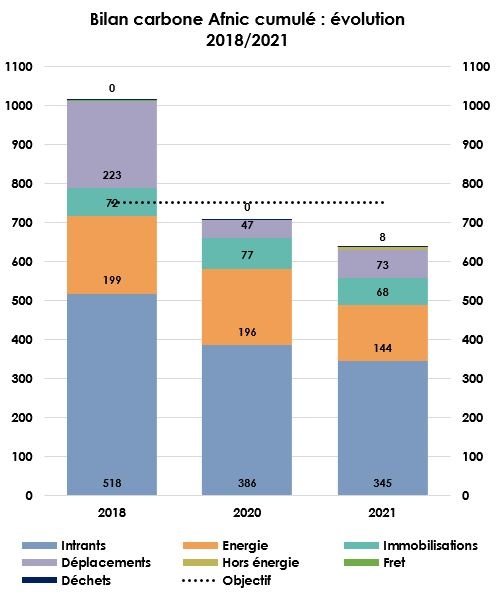
\includegraphics[width=\textwidth]{paper/figures/EvolutionCarbone}
      \caption{Evolution du bilan carbone de l'Afnic}
      \label{fig:evolutionCarbone}
  \end{minipage}
\end{figure}


\section{Qu'est-ce que le DNS}
Le DNS ou Domain Name System (Système de Nom de Domaine en français) est une partie critique au fonctionnement d’internet comme on le connais aujourd’hui.

Son usage principal est de transformer un Nom de Domaine (voir image en dessous) en une adresse IP qui est utilisable pour la transmission.

\begin{figure}[htbp]
  \centering
  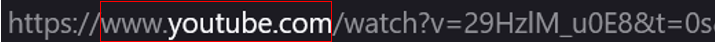
\includegraphics[width=\textwidth]{paper/figures/domainName}
  \caption{Nom de domaine}
  \label{fig:domainName}
\end{figure}

Pour cela, lorsque l’on essaye d’accéder à un site internet (par exemple www.afnic.fr), l’ordinateur envoie une requête dns a son résolveur dns (1).
Ensuite il y a deux cas possibles :

Soit le résolveur n’a pas le Nom de Domaine que l’on demande en mémoire, dans ce cas il doit le trouver de manière récursive.

Il commence par demander aux "\glspl{rootserver}" (2) qui le redirige vers les \glspl{autoritativeserver} sur le \GLSpl{tld} en question. (3)

Ensuite il demande a ces serveurs (4), qui le redirigent vers les \glspl{autoritativeserver} sur la partie suivante du nom de domaine (afnic.fr dans notre cas). (5)

Et il continue jusqu’à trouver le \gls{autoritativeserver} sur le nom qui lui répondra l’adresse ip correspondante. (6)(7)

Finalement une fois que le résolveur connais l'adresse IP corespondant au Nom de Domaine, il la renvois au client (8) qui peut finalement accéder au service souhaité (9)

\begin{figure}[htbp]
  \centering
  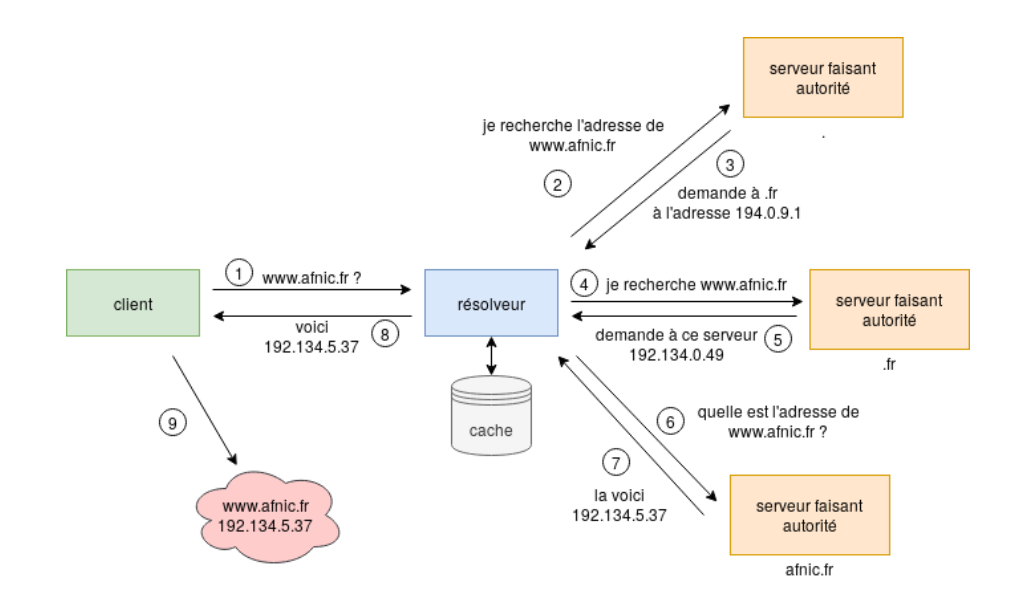
\includegraphics[width=\textwidth]{paper/figures/resolver}
  \caption{Fonctionnement d'un résolveur}
  \label{fig:resolver}
\end{figure}

Si le résolveur connaît déjà l’adresse ip du nom de domaine demandé, il peut répondre directement et sauter les étapes 2 à 7.

Il est aussi possible que le résolveur connaisse déjà une partie du nom de domaine (par exemple on demande zimbra.afnic.fr), dans ce cas il peut directement demander aux serveurs faisant autorité sur la dernière partie commune et sauter les étapes 2 à 5 ce qui divise par deux le nombre de requêtes nécéssaires.

Comme dit plus tôt, un Résolveur fait l’interface entre les clients et les différents serveurs faisant autorité. Ces serveurs intermédiaires ont de nombreux avantages par rapport à faire toutes les requêtes soi-même, principalement au travers de son mécanisme de mémoire (ou Cache).

Premièrement cela réduit le délai de réponse ce qui est très important car le délai des requêtes dns est un des facteurs les plus importants dans la fluidité de navigation sur internet (surtout de nos jours où les connections internet sont de plus en plus rapide). Les résolveurs permettent de réduire le délai de réponse pour plusieurs raisons, la mémoire qui diminue le nombre de requêtes intermédiaires à faire et le fait que les datacenters dans lesquels sont ces serveurs ont des connections internet bien plus rapides que ce qu’un particulier peut obtenir.

Ensuite, cela réduit de façon significative la charge sur les serveurs faisant autorité réduisant les coûts (financiers et environnementaux) de l’infrastructure internet.

Le résolveur dns est généralement assigné en se connectant a un réseau internet, c’est généralement un serveur géré par l’opérateur (Orange, Free, SFR, Bouygues, etc) pour les particuliers et un serveur interne a l’organisation pour les professionnels.

Il existe aussi un certain nombre de résolveur publics (gratuits ou payants) proposant une meilleure vitesse, confidentialité ou même différents services tels que le blocage de publicités, de contenu pornographique ou autre.

Parmi les plus connus on trouve, Google (8.8.8.8), Cloudflare (1.1.1.1), QuadNine (9.9.9.9) et OpenDNS (208.67.222.222).

\section{Un ancien système}
Bien que le protocole DNS soit critique au fonctionnement d’internet, il est très vieux (la RFC 1034 le définissant date de 1987 \cite{dnsRFC}) et il n’est pas vraiment possible de le modifier pour des raisons de compatibilité avec les anciens équipements encore connectés à internet (il n’est pas rare que des équipements critiques soient très anciens notamment dans l’armée, le milieu hospitalier ou l’industrie).

\section{les différentes évolutions}
Sachant qu’il n’est pas possible de modifier le protocole dns directement, d’autres protocoles alternatifs ont été développés pour palier aux différents problèmes qui sont apparus.
\subsection{DoTCP}
Le DoTCP \cite{dotcpRFC} a été le premier protocole alternatif qui est apparu pour palier a la limite de taille dans les réponses DNS, avec l’ajout de l’ipv6, de l’expansion des informations que l’on peut stocker dans le DNS et le développement du DNSSEC, les réponses sont devenues de plus en plus longues et se retrouvent limités par la taille d’un paquet UDP (protocole utilisé par le DNS basic) soit 65,507 bytes.

Le protocole TCP lui permet de séparer un message en plusieurs paquets et permet outre la limite de taille de paquet. Ce protocole a aussi l’avantage de permettre plus de gestion d’erreur et de retransmission en cas de problème sur le réseau.

\subsection{DNSSEC}
Le DNSSEC \cite{dnssecRFC} est une adition au protocole DNS qui permet d’authentifier cryptographiquement la réponse reçue afin d’être sûr qu’elle a bien été renvoyée par le serveur ayant autorité et non par un tiers malicieux.
Cette évolution repose généralement sur les autres protocoles permétant de plus grandes réponses DNS dû a la taille des signatures cryptographiques.

\subsection{DoT}
Le protocole DoT \cite{dotRFC} (DNS over TLS) permet de chiffrer les requêtes DNS via chiffrement TLS (même méthode qu’utilisé pour chiffrer les requêtes http en https).

C'est le premier protocole permétant d’empêcher les intermédiaires (notamment l’opérateur internet ou simplement quelqu’un sur le même réseau) de pouvoir voir tout le trafic dns et donc tous les sites accédés, cependant cela a pour coût la rapidité car l’ajout d’une couche de chiffrement rend la requête plus lourde a traiter pour le client et le serveur.

\subsection{DoH}
Finalement le DoH \cite{dohRFC} (DNS over Https) permet de faire des requêtes dns en passant par le protocole https ce qui les rend presque indistinguables du trafic html classique et est donc très difficile a bloquer par des pare-feu ou autre outil de contrôle (il est facile de bloquer le DoT et donc de forcer l’utilisateur à utiliser d’autres protocoles non privés). 

\imtnechapitre{Synthèse des travaux réalisés}
\setcounter{section}{0}
\section{Mission principale}
Ma première mission a été de mettre en place du monitoring sur un résolveur interne à l’afnic.

Pour cela, j’ai commencé par installer un résolveur sur un vps en suivant un guide présent sur le gitlab interne afin de bien comprendre comment les différents programmes qui composent un résolveur fonctionnent et interagissent entre eux.

Ensuite j’ai essayé plusieurs méthodes pour récupérer les données intéressantes, notamment les données de consommation électrique du serveur qui ne sont évidentes à récupérer.
Une solution simple mais très peu précise est de récupérer le uTime (le nombre de cycles du processeur utilisés) des différents programmes afin de voir leur évolution.

Une deuxième solution que j’ai ensuite trouvée est l’utilisation d’un outil appelé Scaphandre qui permet de récupérer directement la consommation électrique du processeur en temps réel. Cet outil bien que très pratique est encore en développement et possède de nombreuses limitations, premièrement il ne peut pas récupérer les données de consommation des cartes graphiques (pas un problème dans notre cas) et il ne marche dans les machines virtuelles (VM) que s’il est aussi installé sur la machine physique et configuré manuellement pour chaque machine virtuelle ce qui n’est pas le cas pour les fournisseurs cloud tels que OVH, Azure (Microsoft), AWS (Amazon) et Google Cloud.

Après avoir tester plusieurs méthodes, j’ai décidé de récupérer les données grâce a Prometheus car l’organisation possédait déjà une instance Prometheus et parce que tous les programmes utilisés peuvent exposer leurs statistiques dans un format compatible.
Une fois l’architecture du système conçue, j’ai dû apprendre le fonctionnement des dockers afin de pouvoir intégrer les nouveaux outils ainsi que les changements de configuration nécessaires a leur fonctionnement, a la récupération de statistique et a l’activation des interfaces Prometheus.

Après plusieurs cycles de modifications afin de que tout marche comme prévu à l’intérieur des différents dockers.

En parallèle, j’ai demandé l’ouverture des flux entre le serveur Prometheus et le résolveur (sur les différents ports donnant accès aux interfaces Prometheus).

Une fois tous les flux fonctionnels, j’ai créé un nouveau dashboard (tableau de bord) dans le grafana interne (déjà relié au serveur Prometheus) et fait des graphiques avec les informations intéressantes :

\begin{itemize}
    \item La consommation totale du serveur
    \item La consommation des différents processus du résolveur (il y a d’autres services tournant sur le même serveur)
    \item Le nombre de requêtes en Cache/Pas en Cache par seconde
    \item Le nombre de requête de chaque type (DoH,DoT,Dns) par seconde
\end{itemize}

\begin{figure}[htbp]
  \centering
  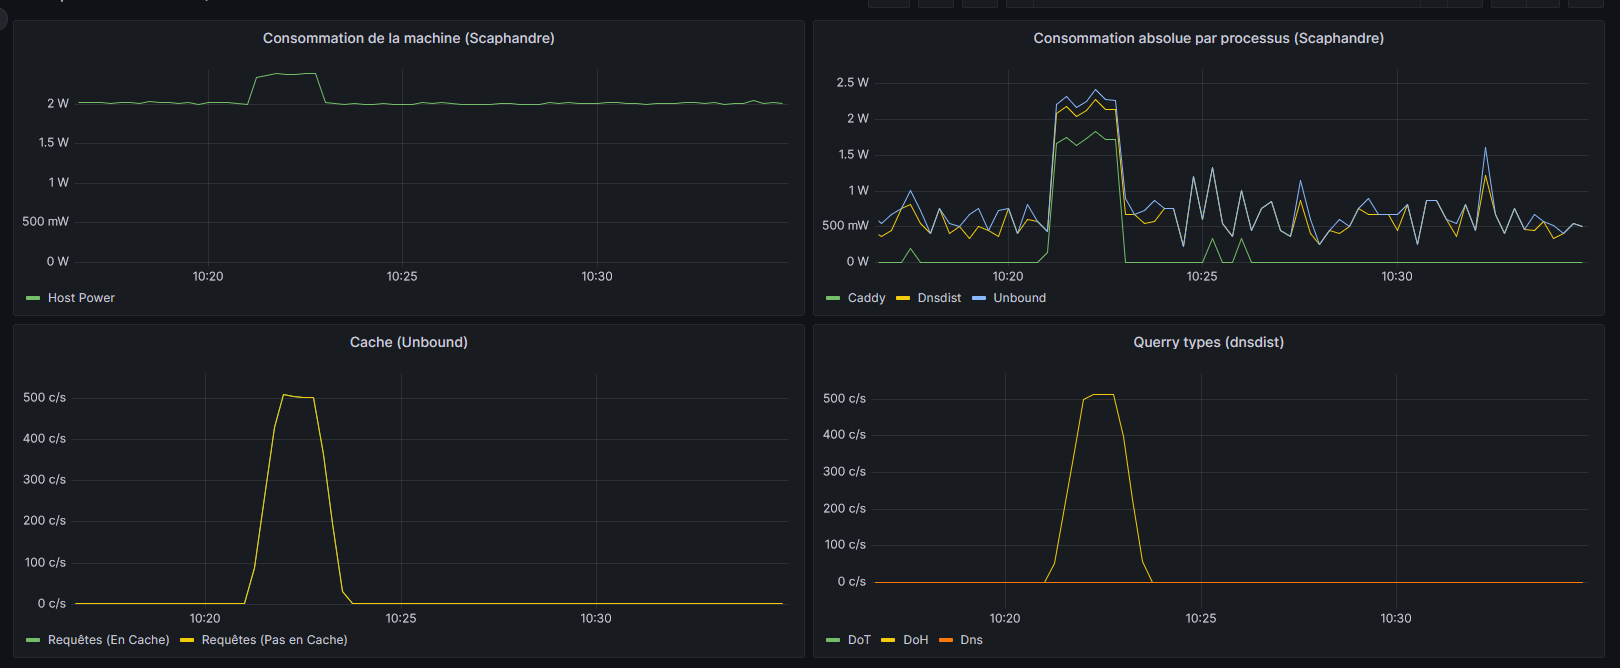
\includegraphics[width=\textwidth]{paper/figures/grafanaDNS.png}
  \caption{Tableau de Bord Grafana}
  \label{fig:grafanaDNS}
\end{figure}


\section{Outil de génération de requêtes DoH}
A côté de ça, j’ai développé un simple outil web (page en pur html+js, aucune interaction côté serveur) afin de pouvoir tester le résolveur DoH sous charge.
Il permet de rentrer l’adresse du résolveur, les types d’enregistrement DNS a demander, et le délai entre chaque requête. J’y ait plus tard ajouté la possibilité d’importer une liste de noms de domaines via csv afin de remplacer celle par défaut (Top 1000 Alexa) 

\begin{figure}[htbp]
  \centering
  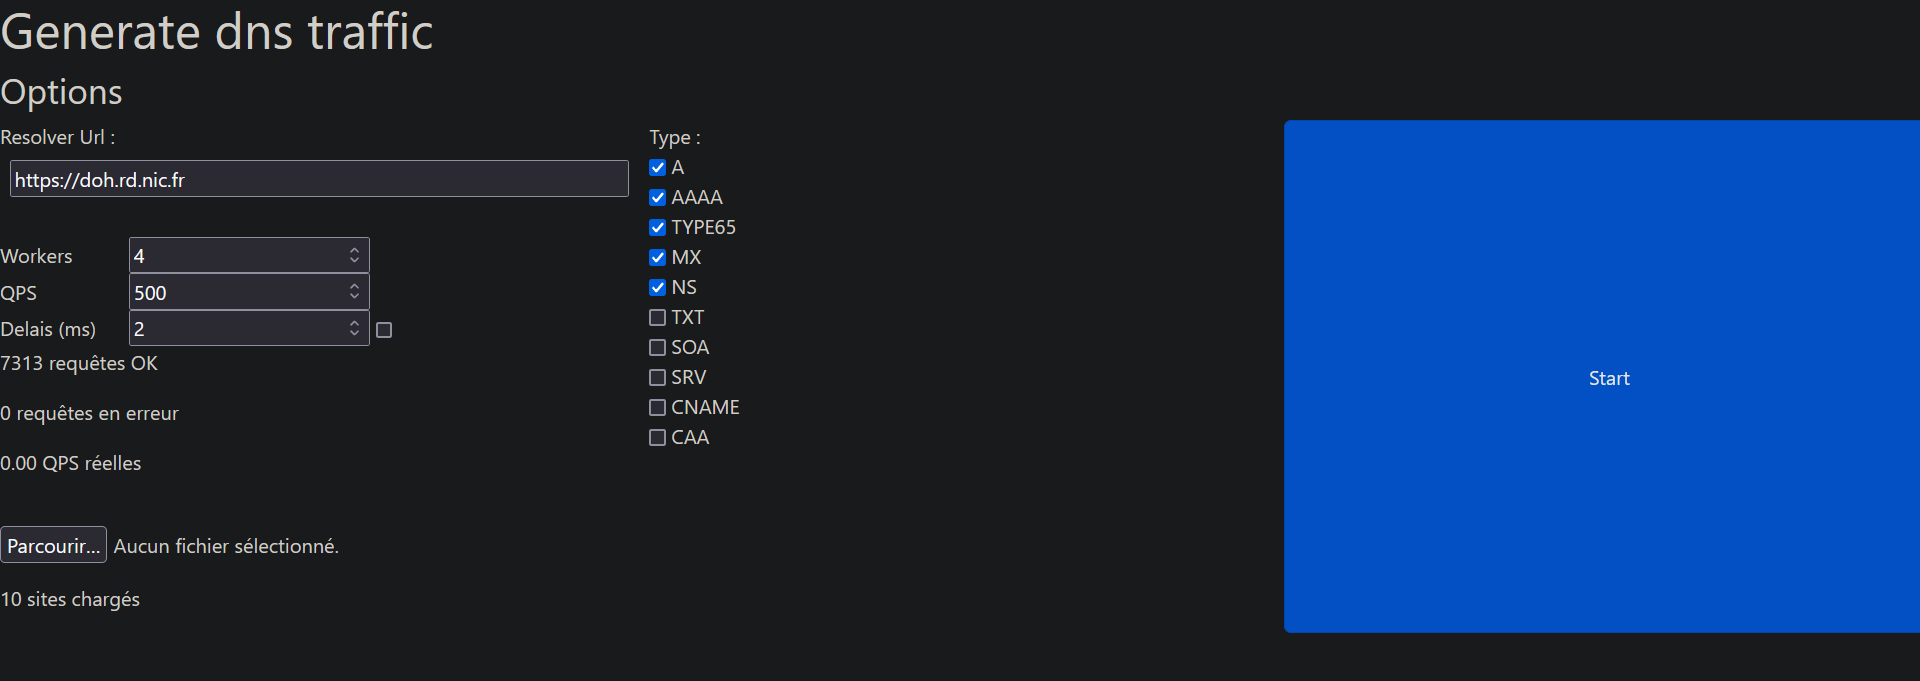
\includegraphics[width=\textwidth]{paper/figures/outilDoh.png}
  \caption{Visuel de l'outil de génération de requêtes DoH}
  \label{fig:outilDoh}
\end{figure}


J’ai ensuite créé un « virtual host » sur le serveur web interne et ajouté l’enregistrement correspondant dans le résolveur dns interne afin de pouvoir y accéder facilement depuis le réseau de l’organisation.

 
\section{Interface entre Wattmètres et Grafana}

Une autre de mes missions a été d’interfacer les Wattmètres (APCs) installés dans les baies de serveurs dans les deux principaux datacenters (TH3 et Marseille) utilisés pour la production (principalement \gls{anycast} DNS \todo{vrai ?)}) avec le système de monitoring central (Prometheus \verb|&| Grafana) afin de remplacer Observium qui bien qu'ayant une intégration native avec le protocole SNMP (Simple Network Management Protocol) utilisé pour communiquer avec les APCs n'est pas du tout ergonomique et demande de nombreux clics pour récupérer les informations nécessaires sans possibilités de les centraliser.

Le principal problème avec le fait d'interfacer des outils snmp avec prometheus est que Prometheus "\Gls{scrape}" les données, c'est a dire qu'il vas chercher "Des données" toutes les x secondes/minutes et stocke ce qu'il trouve alors que pour récupérer des données via le protocole SNMP, il faut demander les données que l'on souhaite. Il y a aussi le fait que les données renvoyés par SNMP ne sont pas dans un format compatible avec SNMP.

Pour résoudre ce problème, j'ai trouvé un outil appelé snmp\_exporter qui permet de faire la liaison entre les deux. Quand il reçois une requête de Prometheus (qui contient l'adresse de l'appareil SNMP cible ainsi que le nom du "Module" a utiliser), il vas chercher dans sa config le Module correspondant qui indique quelles sont les données souhaités puis vas les demander via SNMP a l'appareil, les met en forme afin qu'elles soient lisibles par Prometheus et finalement renvois cette réponse avec les données correctement formatés a Prometheus.

\todo{lien vers la doc}

\begin{figure}[htbp]
  \centering
  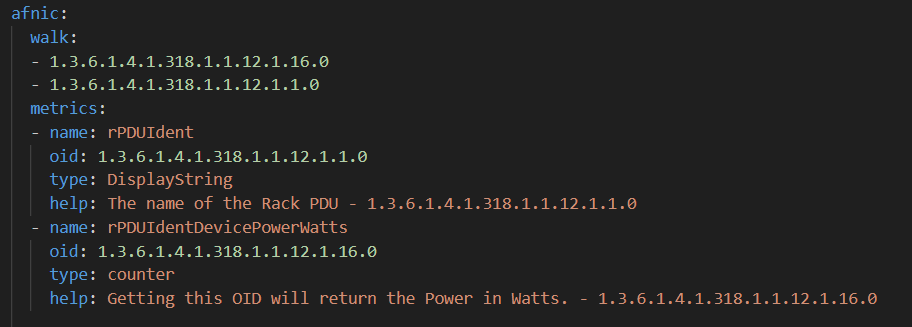
\includegraphics[width=\textwidth]{paper/figures/exempleConfigSNMP.png}
  \caption{Exemple de fichier de configuration de snmp\_exporter}
  \label{fig:exempleConfigSNMP}
\end{figure}

\todo{Rajouter nomad ?}

Une fois tout cela fait, on peut directement afficher toutes ces données sur Grafana :
\begin{figure}[htbp]
  \centering
  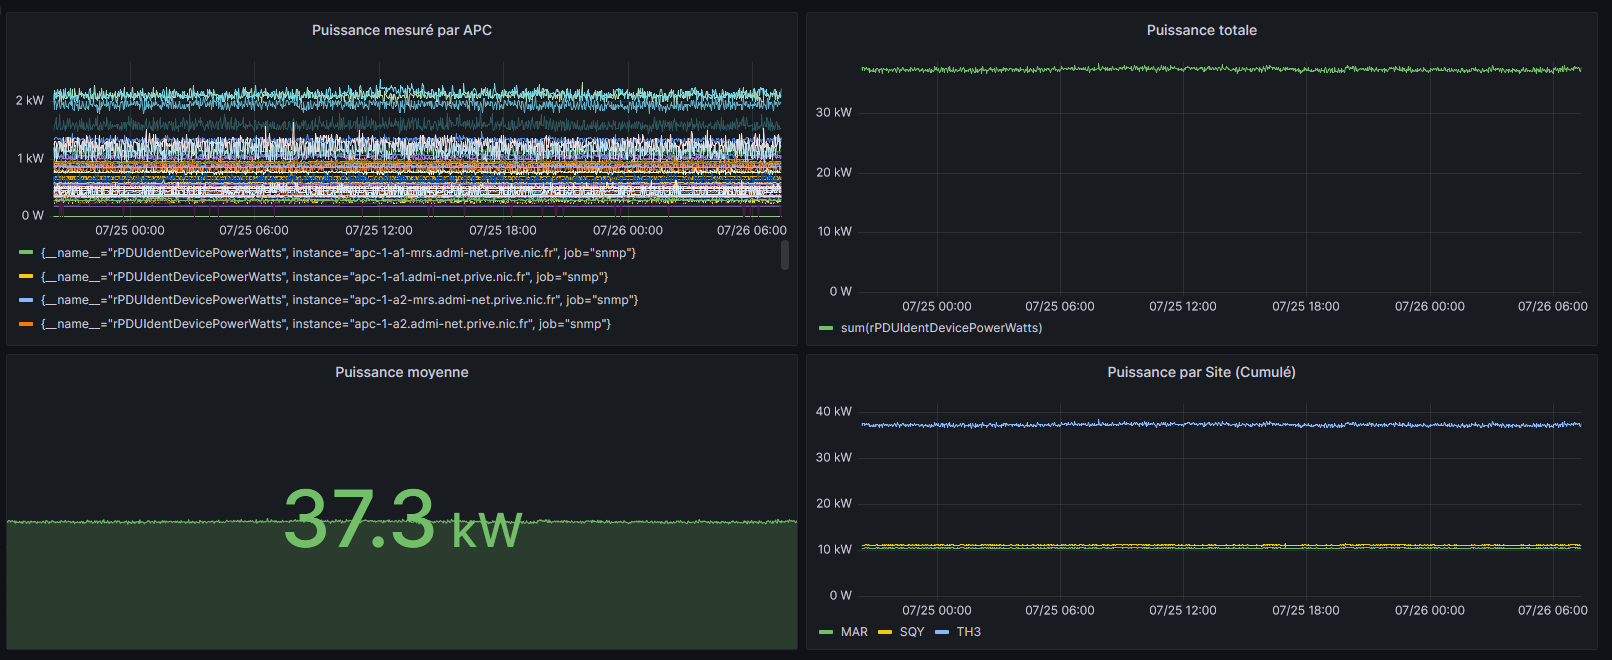
\includegraphics[width=\textwidth]{paper/figures/GrafanaAPC.png}
  \caption{Tableau de Bord Grafana APCs}
  \label{fig:GrafanaAPC}
\end{figure}

\section{Analyse des données récupérés}

Avant de commencer a analyser les données récupérés, il est important de préciser ce qu'elles représentent.
Ici nous allons uniquement étudier les données de consommation de serveurs (la machine physique) en corélation avec le nombre de requêtes dns traités.
Toutes les autres sources de consommation tels que les routeurs, firewall ou tout autre intermédiaire par lesquels passent les requêtes dns ne sont pas pris en compte.

Pour le résolveur, nous avons utilisé un serveur Bare Metal (gamme où la totalité d'un serveur est loué et non seulement un machine virtuelle) Rise-APAC-1 \todo{a vérifier, correspond a part pour modèle CPU, probablement plus disponible} avec ces caractéristiques :
\begin{itemize}
    \item Intel Xeon E3-1270v6 (4 coeurs/8 threads, 3.8GHz)
    \item 32 Go de RAM ECC DDR4
    \item SSD NVMe
    \item 500Mb/s de Bande passante
\end{itemize}

Cette configuration est bien au delà de ce qui est nécessaire pour un résolveur dns de faible ampleur cependant c'est une des plus basses qui correspondait a nos besoins :
\begin{itemize}
    \item Bare Metal du fait des limitations de Scaphandre
    \item Bande passante conséquente afin que ça ne soit pas un facteur limitant lors des mesures
\end{itemize}


\subsection{Résolveur}

\begin{figure}[ht]
  \noindent
  \begin{minipage}{.65\textwidth}
Pour ce qui est du résolveur, on remarque deux parties spécifiques :

Pour des volumes relativement faibles, la consommation électrique du serveur est constante et ne diffère pas de la consommation de référence (quand le serveur ne fait rien).

Pour des volumes plus élevés (plusieurs centaines voir milliers de requêtes par seconde), la consommation est plus ou moins lié de façon linéaire au nombre de requêtes reçues par seconde.

Ceci est lié au cpu (donc les données dépendent fortement du modèle de processeur utilisé) dont la consommation n'est pas linéairement lié a son utilisation. 
  \end{minipage}
  \hfill
  \begin{minipage}{.30\textwidth}
    \centering
      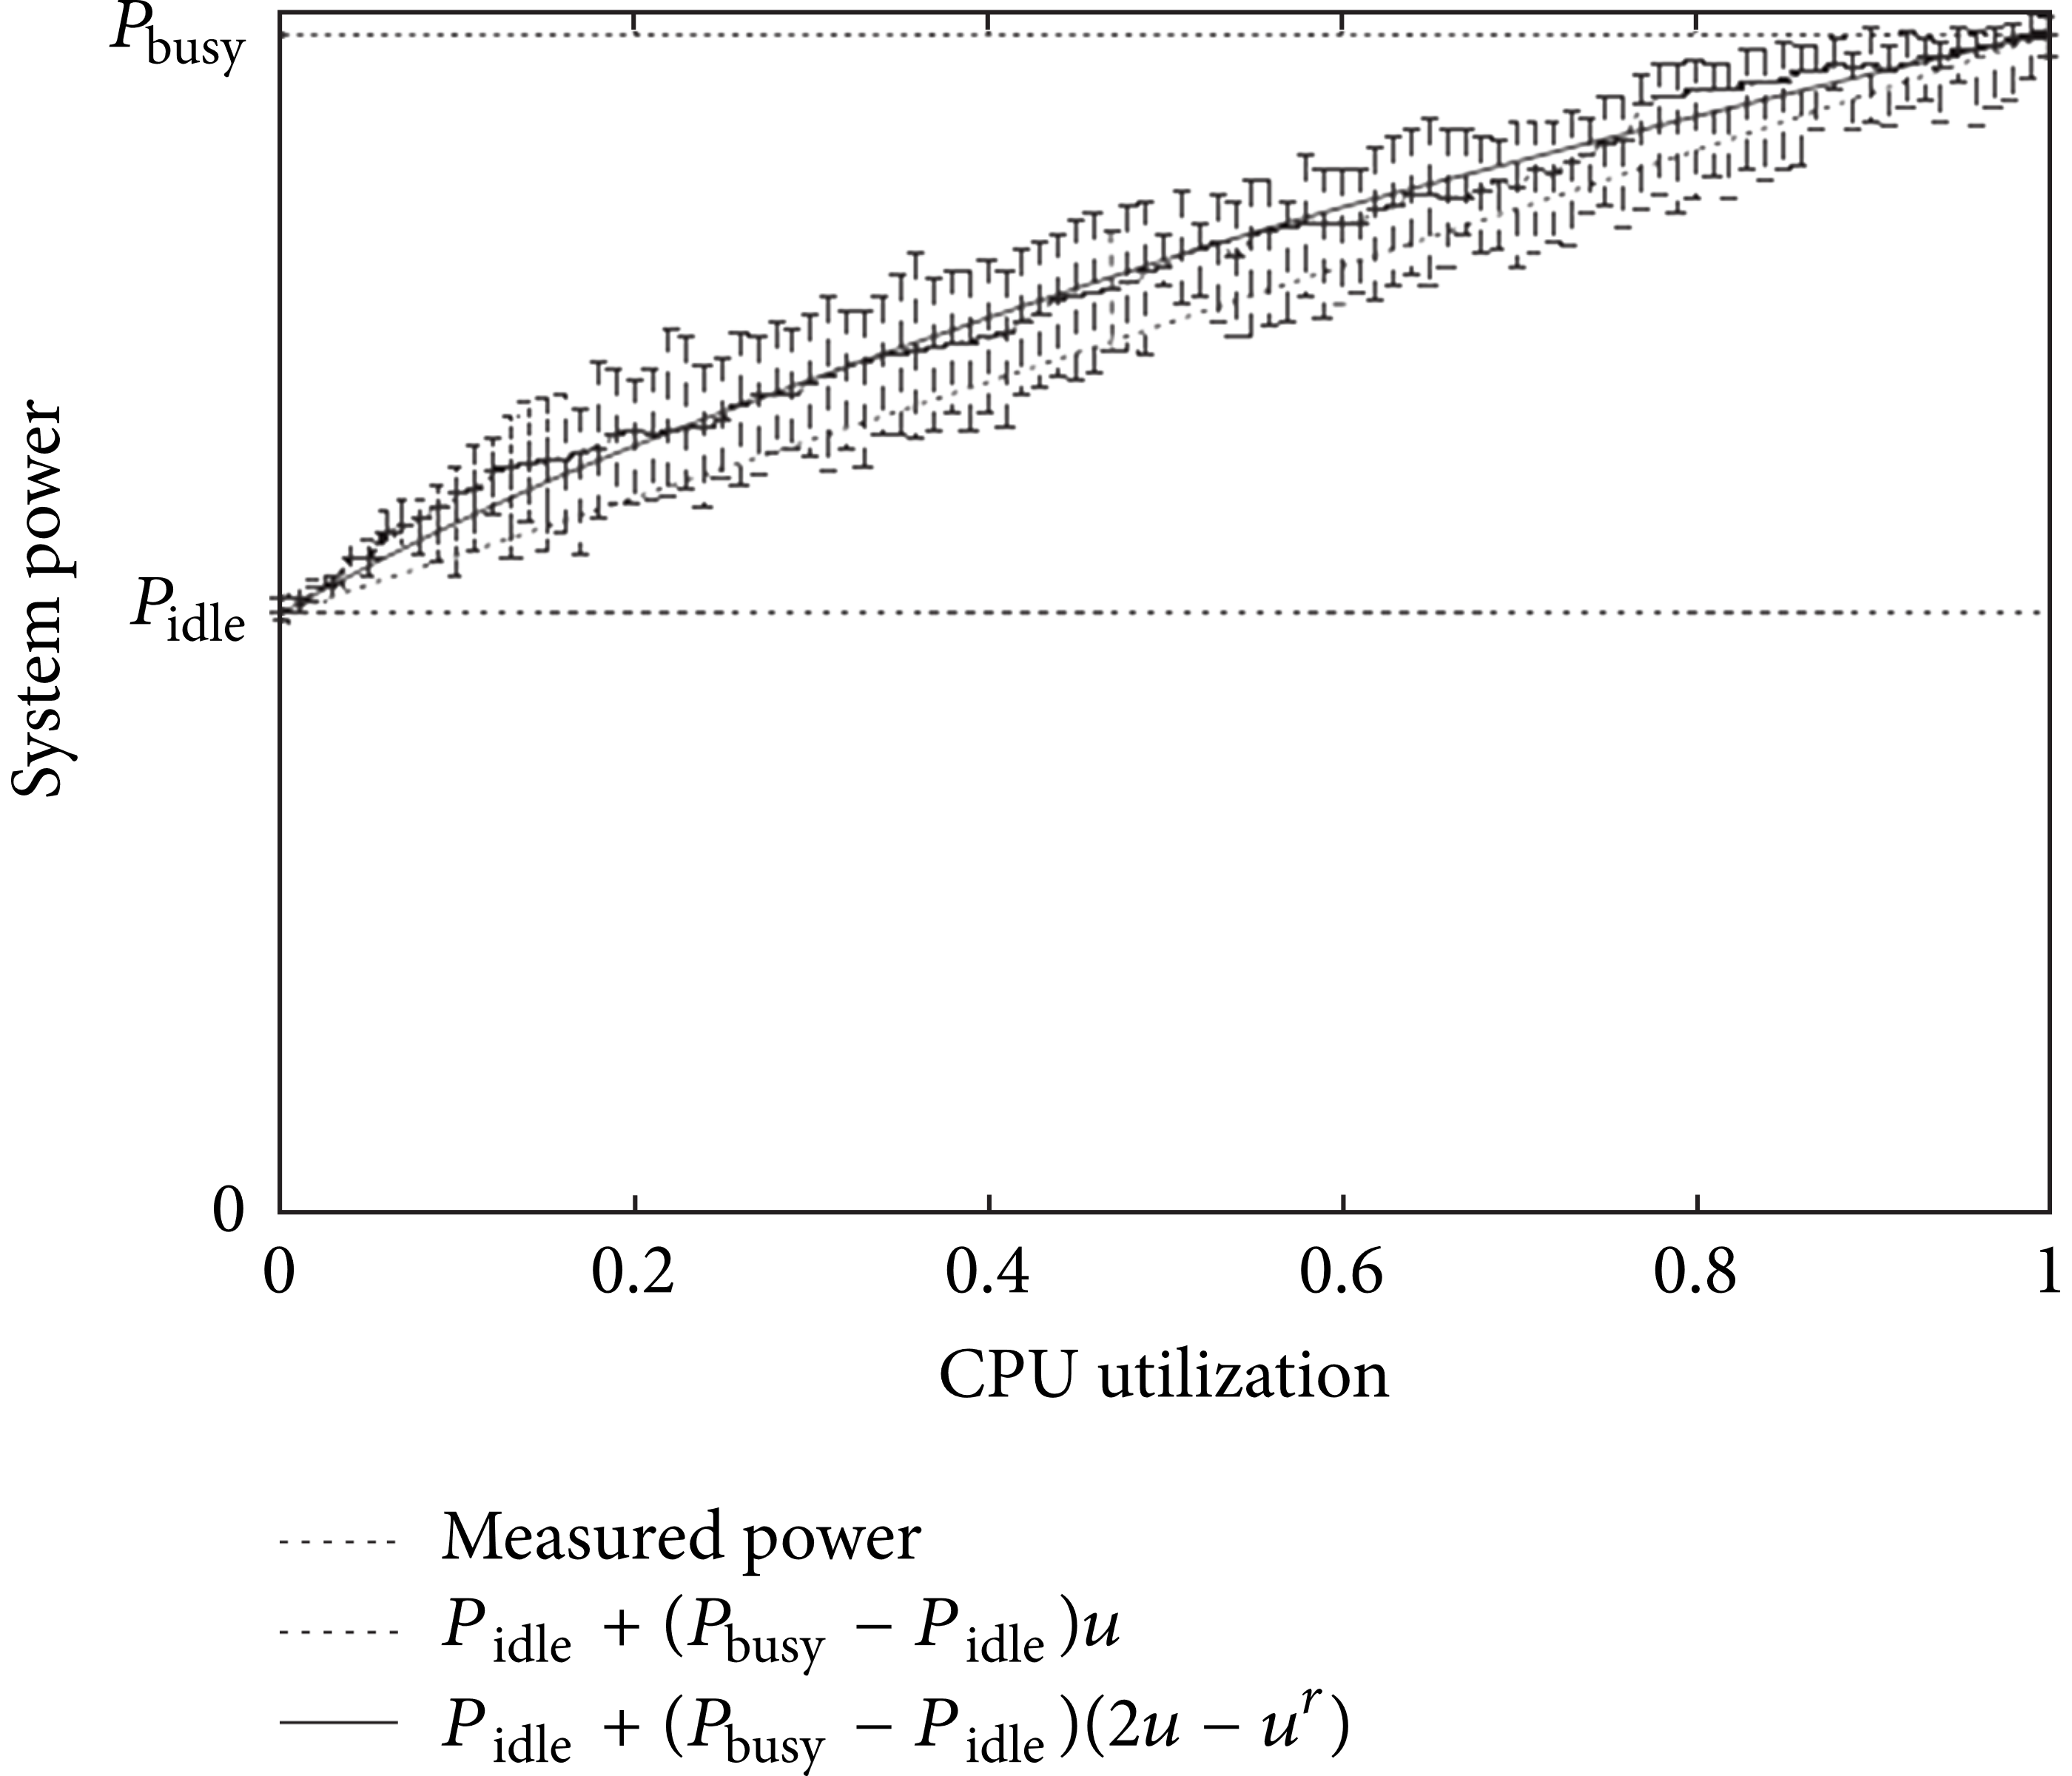
\includegraphics[width=\textwidth]{paper/figures/exempleCPUcurve.png}
      \caption{Exemple de courbe de consommation d'un processeur de serveur \cite{cpuGraph}}
      \label{fig:exempleCPUcurve}
  \end{minipage}
\end{figure}

Ceci fait qu'il est préférable de faire tourner un petit résolveur dns (par exemple pour une entreprise de taille moyenne) sur un plus petit serveur que celui utilisé pour les tests ou encore mieux sur une machine virtuelle afin de partager la consommation avec d'autres applications car plus la machine est utilisé moins elle consomme par cycle cpu "utile".

C'est dans ce genre de cas que des infrastructures telles que Nomad qui déployent les différents services automatiquement en fonction de l'utilisation des différents serveurs peuvent être très efficace.
Il faut cependant tenir compte de la possibilité de pics soudain d'utilisation et de marges de redondance en cas d'échec d'un ou plusieurs serveurs.

\subsection{Nuage Anycast}
Pour ce qui est de la consommation du \gls{anycast}, elle est très constante malgré un volume de requêtes variant du simple au double durant la journée.
\todo{voir pourquoi ?}

\begin{figure}[ht]
  \noindent
  \begin{minipage}{.55\textwidth}
Ici, nous sommes dans une situation demandant beaucoup de redondance et de stabilité dû a l'importance du service fournit (si l'infrastructure ne répond pas, aucun site web ou service en .fr n'est accessible une fois le cache des différent résolveurs expiré)

En conclusion, on rejoins l'idée que la consommation électrique n'est pas directement proportionnelle au nombre de requêtes mais est constante.
(Il faut néanmoins prendre en compte que le volume de requêtes influence le nombre d'équipement réseau et serveur nécessaires mais cette différence n'est présente qu'au niveau macroscopique). \cite{blogStephaneConsoElec}

Il est tout de même intéressant de remarquer qu'une part très importante des requêtes dns envoyés lors d'une session de navigation internet classique est constitué de requêtes liés a la publicité et au traçage (notamment sur les sites de journaux qui peuvent causer des dizaines de requêtes en une seule page). Ce phénomène est aussi visible par le fait que dans le top 10 000 OpenPageRank, il y a 3000+ domaines qui sont des sous-domaines de doubleclick.net, la solution de publicité et de traçage de Google. \cite{openPageRank}
  \end{minipage}
  \hfill
  \begin{minipage}{.40\textwidth}
    \centering
      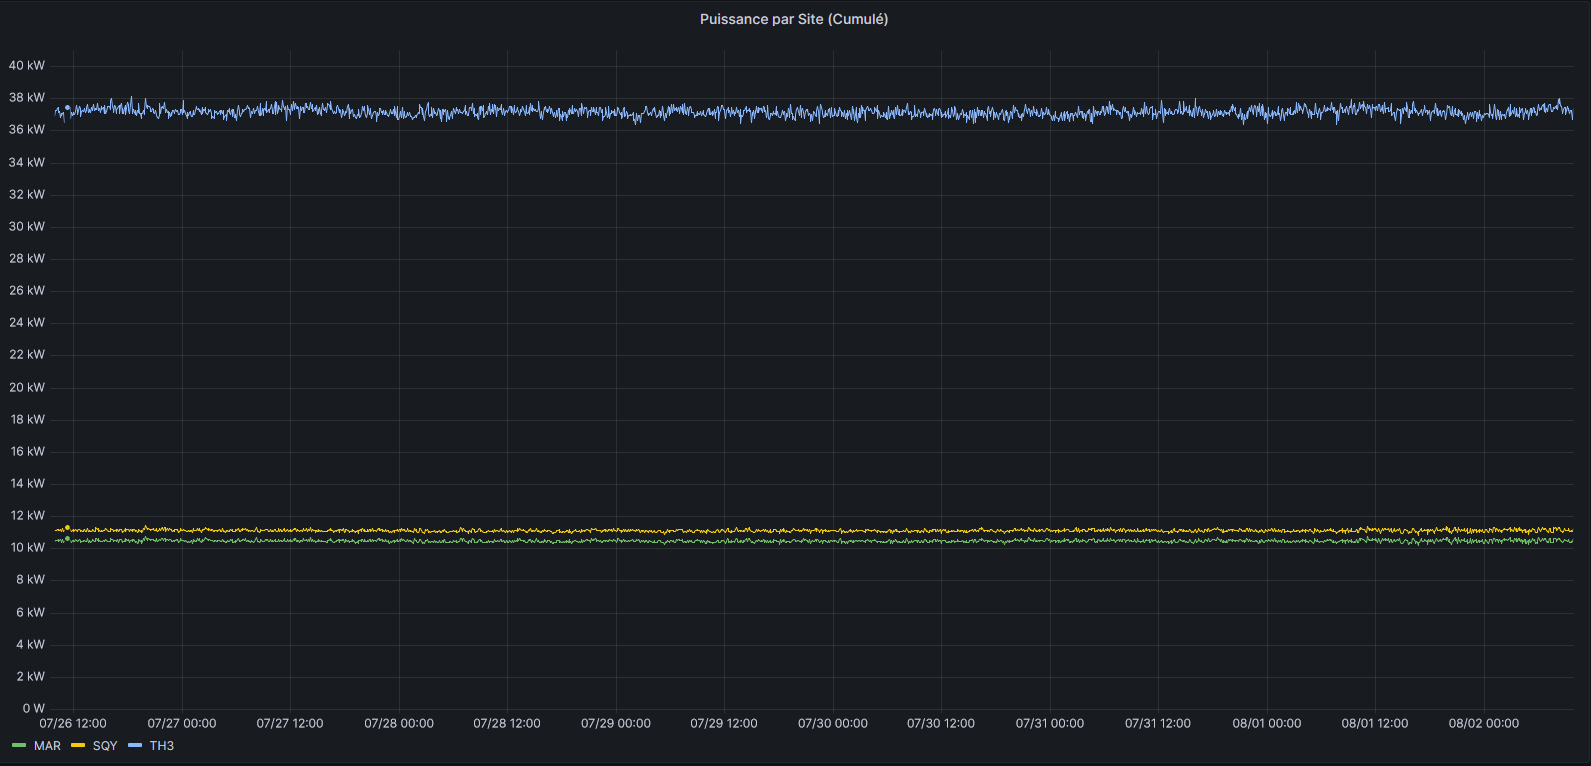
\includegraphics[width=\textwidth]{paper/figures/puissanceParSite.png}
      \caption{Puissance utilisé par site(datacenter)}
      \label{fig:puissanceSite}
  \centering
      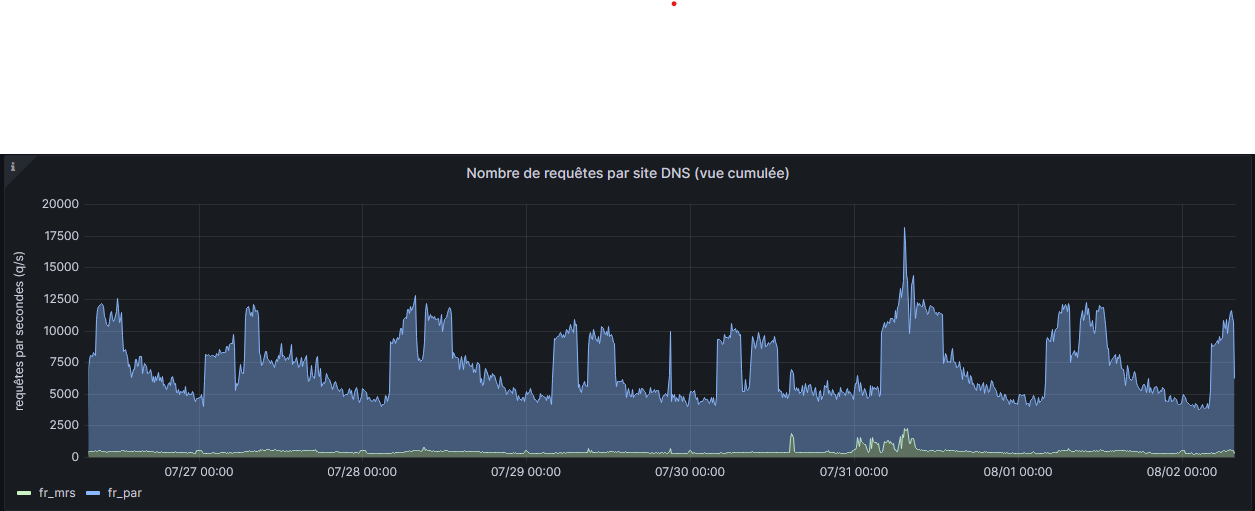
\includegraphics[width=\textwidth]{paper/figures/qpsAnycast.png}
      \caption{Nombre de requêtes par secondes sur le \gls{anycast} de l'afnic}
      \label{fig:QPSAnycast}
  \end{minipage}
\end{figure}

Voir annexe \ref{A:puissanceParSite} et \ref{A:QPSAnycast} pour les graphiques en plus grand
\imtnechapitre{Impressions Personnelles et Acquis}
Lors de ce stage, j'ai découvert plusieurs outils très pratique notement Docker et Docker-compose qui est des solutions clefs en main qui permettent de déployer des programmes (site web, service, logiciel, autre) très facilement et indépendamment de la plateforme. Bien que ce soit pas recommandé pour des grosse infrastructures de production, il y a de nombreux cas où l'utilisation de Dockers est valide.

En dehors de cela, j'ai aussi apris a utilisé Prometheus et Grafana qui sont des outils très utilisés pour récupérer des données de monitoring de nombreuses sources et afficher ces données respectivement. De façon plus transverse, je me suis familiarisé avec des distribution de linux utilisés en production que je n'avais pas encore eu l'ocasion de manipuler tels que RedHat.

En sortant de l'aspect purement technique, j'ai pu développer ma prise de décision et mon autonomie car j'était responsable de faire les choix liés a ma mission (quels outils utiliser comment les implémenter, etc) et devais réfléchir au pour et au contre de chacun. Cela était très intéréssant car dans mes précédants stages j'était généralement restraint a l'infrastructure déjà en place et a des choix déjà faits car je me greffais à un projet déjà existant alors qu'ici je commançait un projet de zéro et c'est moi qui était responsable de faire mes recherches et apporter des solutions aux différents problèmes techniques.

Le mode de travail de l'équipe était aussi nouveau pour moi, le fait d'être dans une équipe où chaque personne travaille sur ses propre projets (certains gros projets avec 2 ou 3 personnes dessus maximum) a fait que j'ai apris et découvert beaucoup de choses lors des réunions d'équipe où beaucoup de sujets était abordés. Cela montre aussi encore plus l'importance d'avoir des documentations claires et complètes car il y en a beaucoup et ils ont généralement été réalisés par une seule personne.

J'ai aussi trouvé je rythme de travail 32h\verb|/|4jours meilleur que 35h\verb|/|5 jours car en comptant le temps perdu chaque jour a lire les emails, faire son planning de la journée et autre, il ne me semble pas avoir d'avoir d'impact conséquent sur le nombre d'heures effectives et le jour non travaillé par semaine est très utile, en dehors du temps libre en plus, c'est aussi l'occasion de faires ses démarches administratives et autres auprès des organismes qui ne sont pas ouvert le weekend.

Ce stage m'a donc permis d'avancer sur mon projet professionnel et m'a conforté dans ma décision de m'orienter vers la partie système/réseau/sécurité de l'informatique et non sur la partie développement pur.

\imtnechapitre{Conclusion}
En conclusion, ce stage m'a donné l'opportunité de développer de nombreuses compétences mais aussi de découvrir un environnement de travail différents de mes autres stages (Travail en entrepot grande entreprise, PME/Startup, Grosse entreprise compta/expertise comptable), une association dans une équipe avec beaucoup d'autonomie.

J'ai aussi pus me familiariser avec des nombreux outils liés a l'infrastructure et au réseau tels que Nomad et Traefik.

Finalement, j'ai pus avoir l'expérience de réaliser un projet en total autonomie avec entière responsabilité de choix sur les différents aspects ce qui de mon point de vue est beaucoup plus représentatif du travail d'un ingénieur que les missions que j'avais éffectués lors de mes précédents stages.


\printnoidxglossaries
\printbibliography[heading=bibintoc]

\pagebreak
\appendix

\imtnechapitre{Annexes}

\begin{figure}[!htbp]
    \centering
      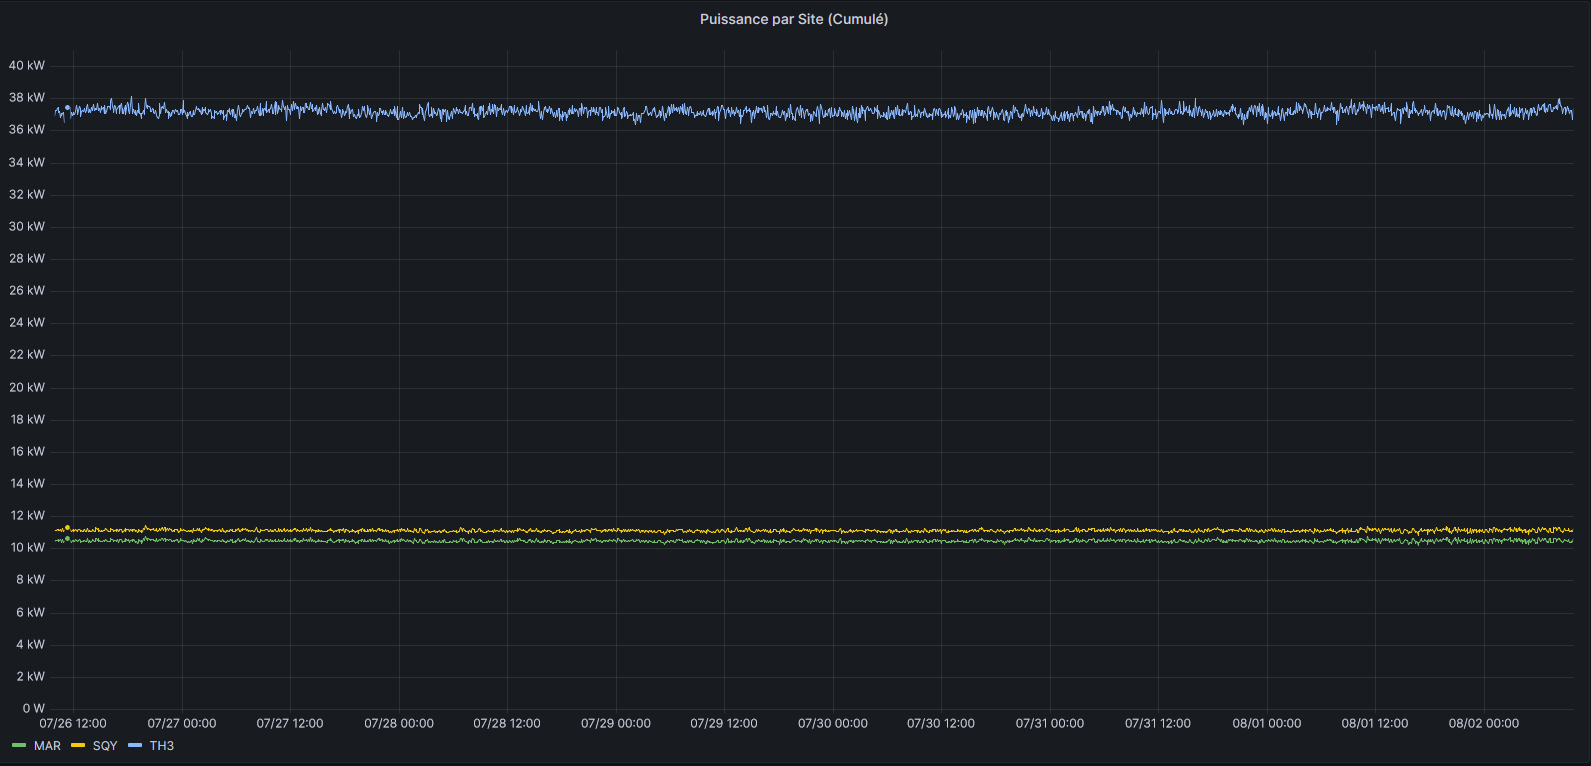
\includegraphics[width=\textwidth]{paper/figures/puissanceParSite.png}
      \caption{Puissance utilisé par site(datacenter)}
    \label{A:puissanceParSite}
\end{figure}



\begin{figure}[!htbp]
    \centering
      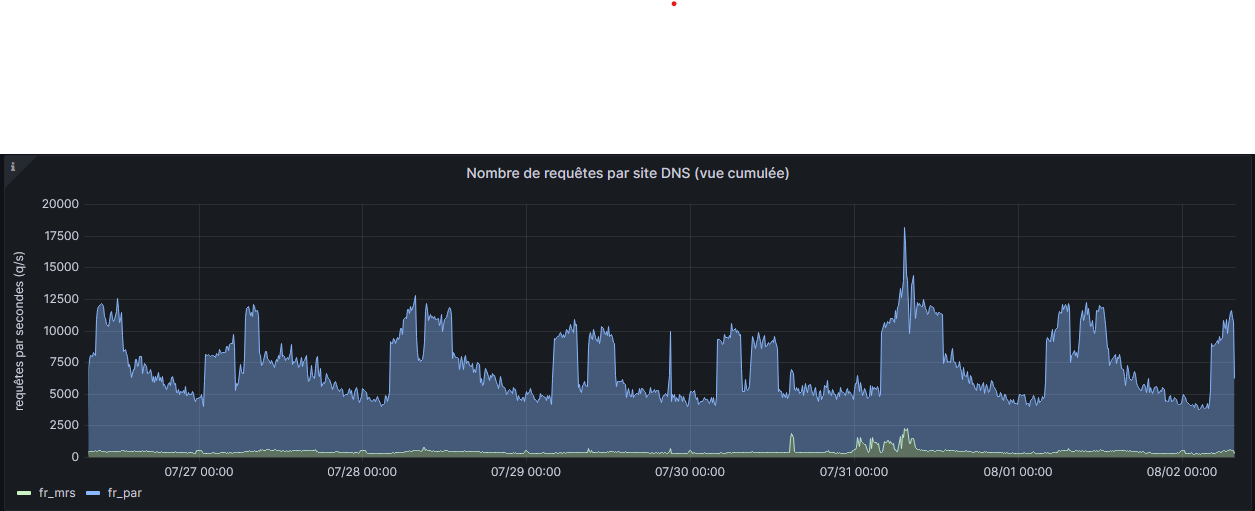
\includegraphics[width=\textwidth]{paper/figures/qpsAnycast.png}
      \caption{Nombre de requêtes par secondes sur le \gls{anycast} de l'afnic}
      \label{A:QPSAnycast}
\end{figure}

\end{document}
